\chapter{VAR-Tool}
\label{ch:main-matter}
  \begin{figure}[H]
    \centering
    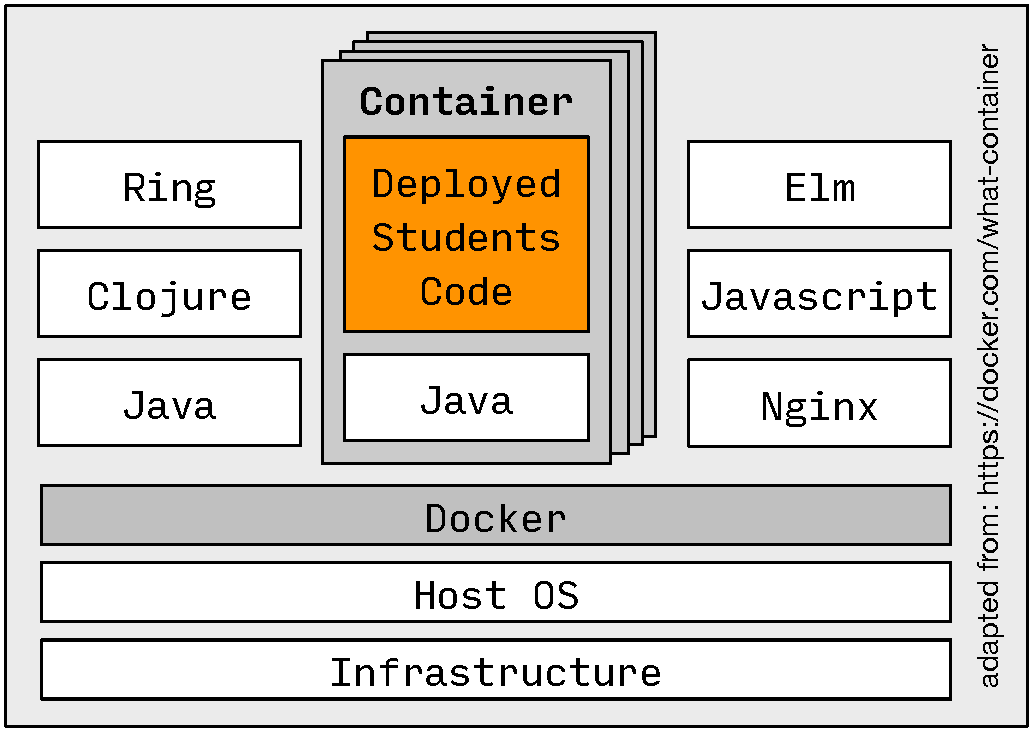
\includegraphics[scale=0.4]{container_intro_centered.pdf}
    \par
    \caption{Container-Übersicht}
    \label{fig:container-intro}
  \end{figure}
  \clearpage

% \section{Analyse}
% \subsection{As-Is}
% \subsection{To-Be}

\section{UI-Mockup}
\begin{landscape}
  \begin{figure}[h]
    \centering
    \fbox{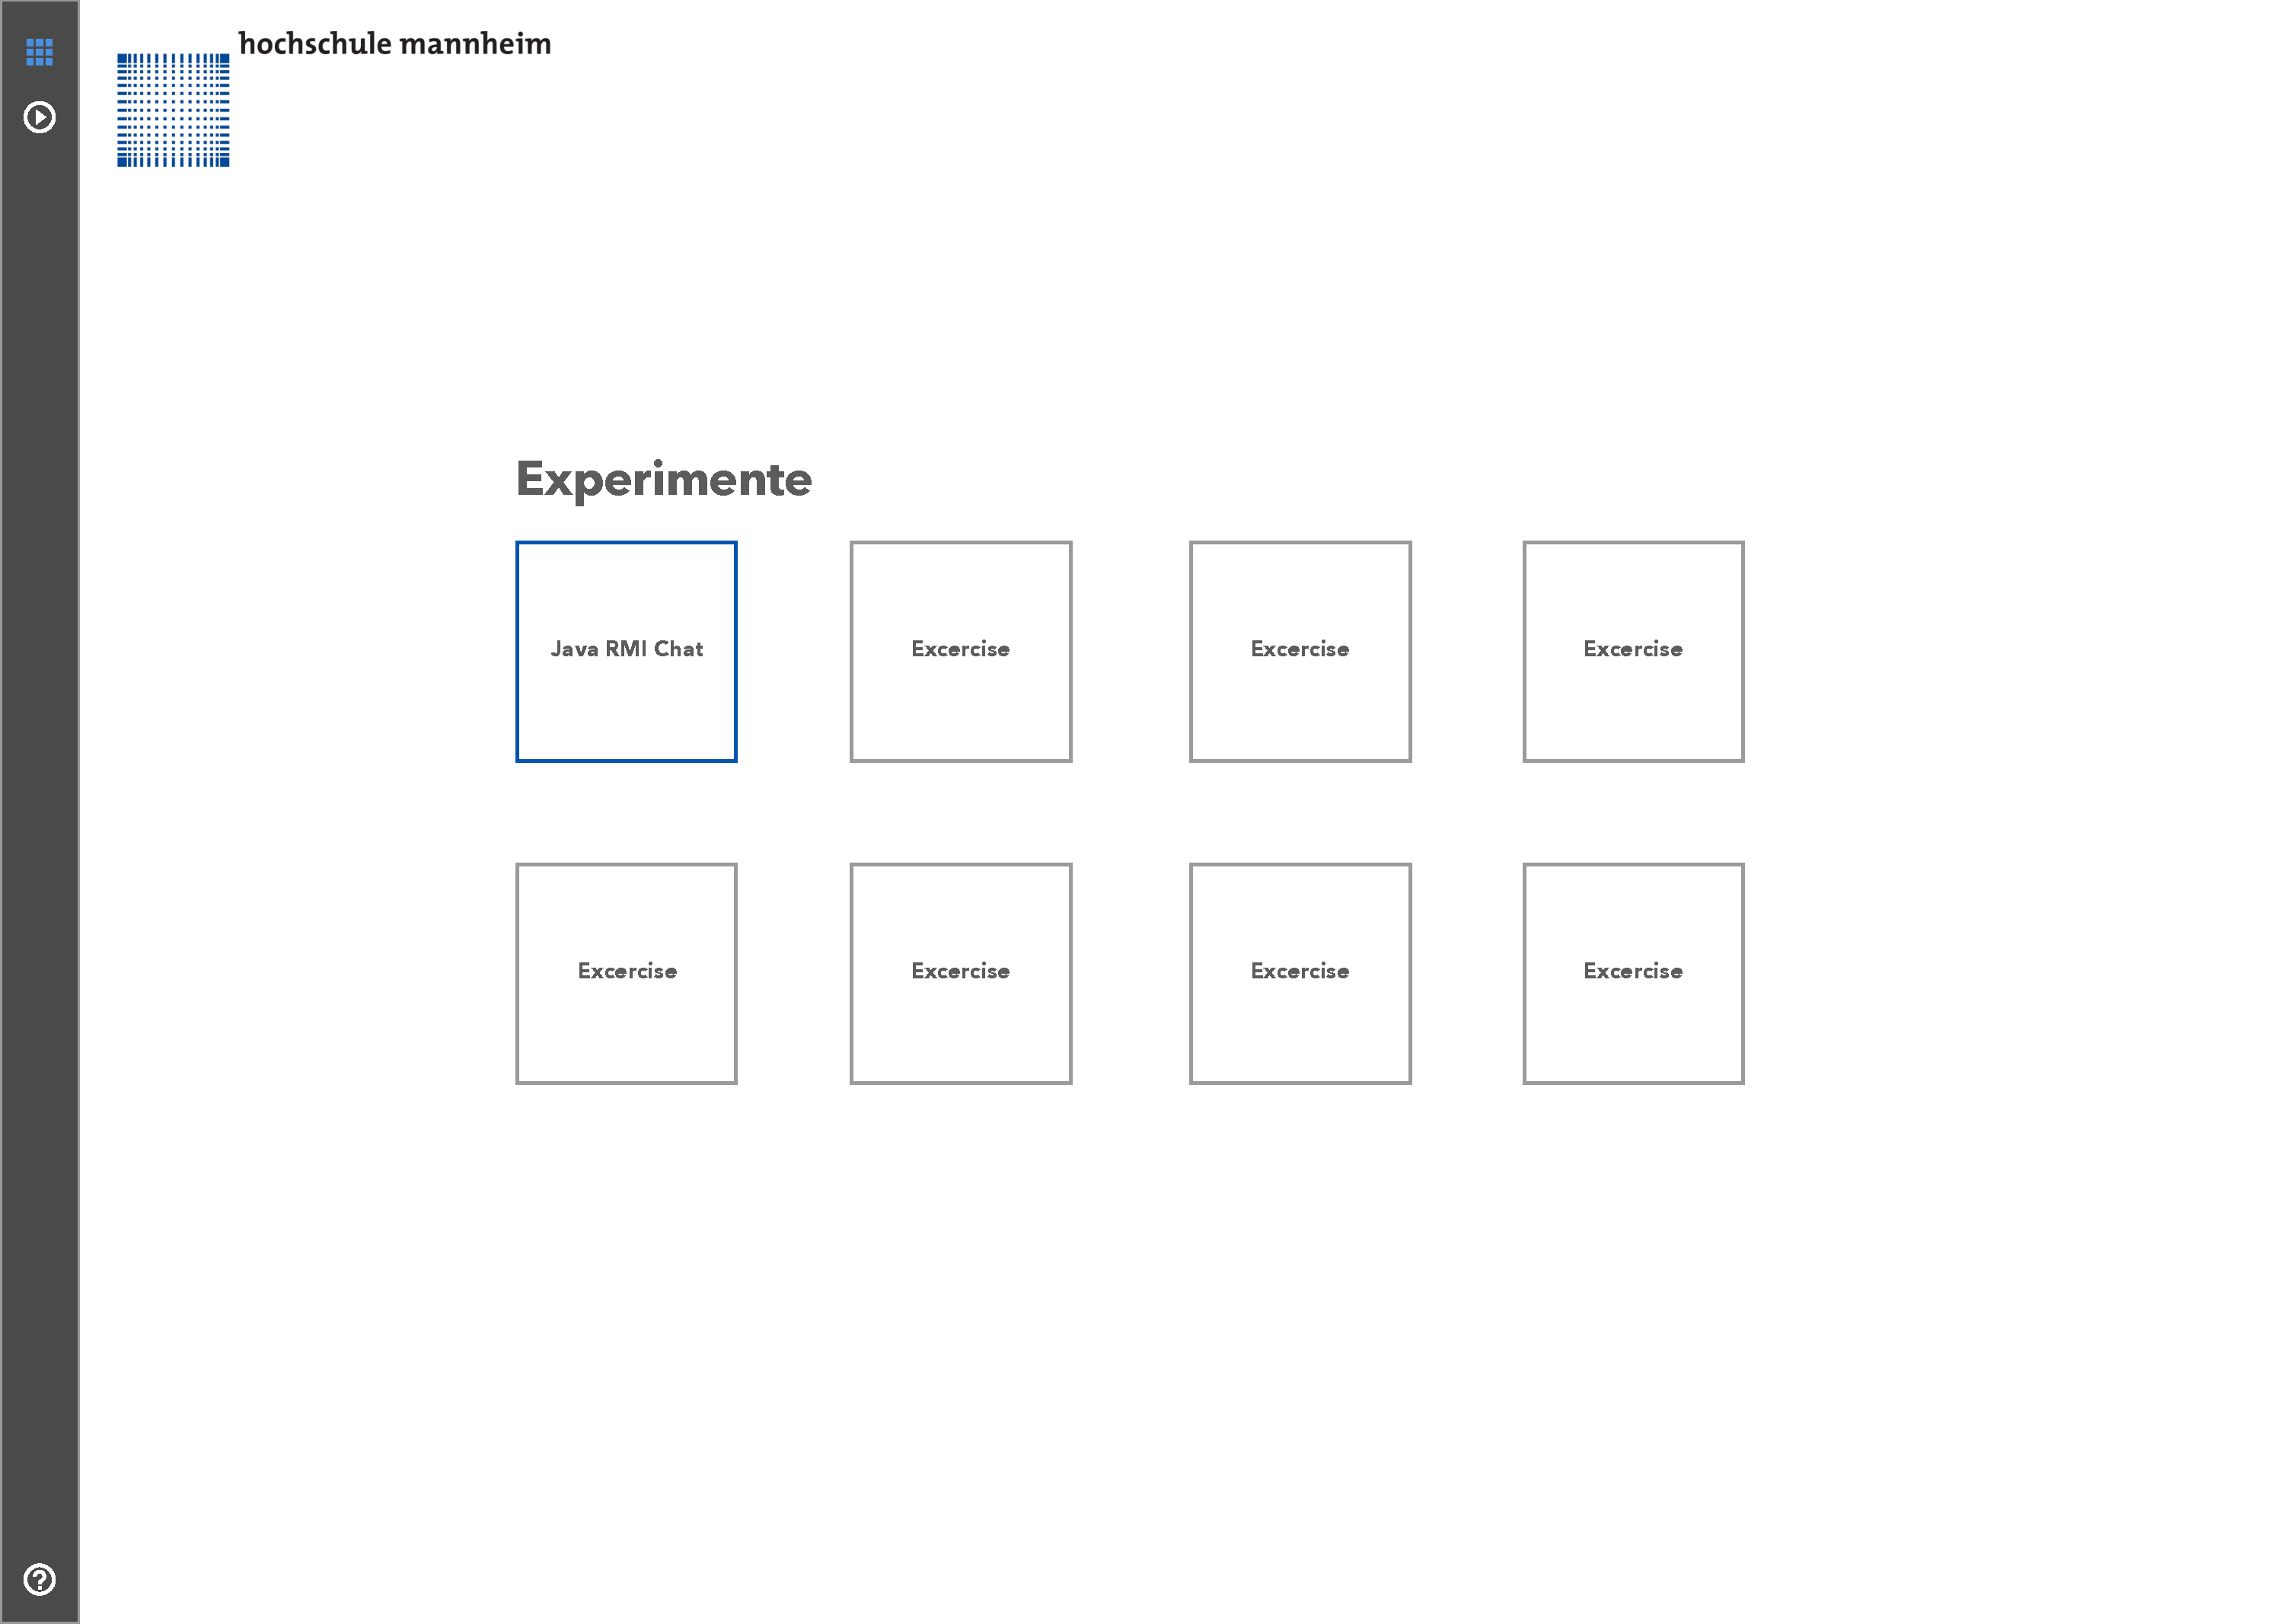
\includegraphics[scale=0.4,page=1]{ui-mockup.pdf}}
    \par
    \caption{UI-Mockup: Übersicht der Experimente}
    \label{fig:ui-mockup-1}
  \end{figure}
  \begin{figure}[h]
    \centering
    \fbox{\includegraphics[scale=0.4,page=2]{ui-mockup.pdf}}
    \par
    \caption{UI-Mockup: Experimentenansicht mit verschiedenen Zuständen pro Instanz}
    \label{fig:ui-mockup-2}
  \end{figure}
\end{landscape}

\section{Architektur}

\subsection{Geschäftsprozesse}
\begin{landscape}
  \begin{figure}[h]
    \centering
    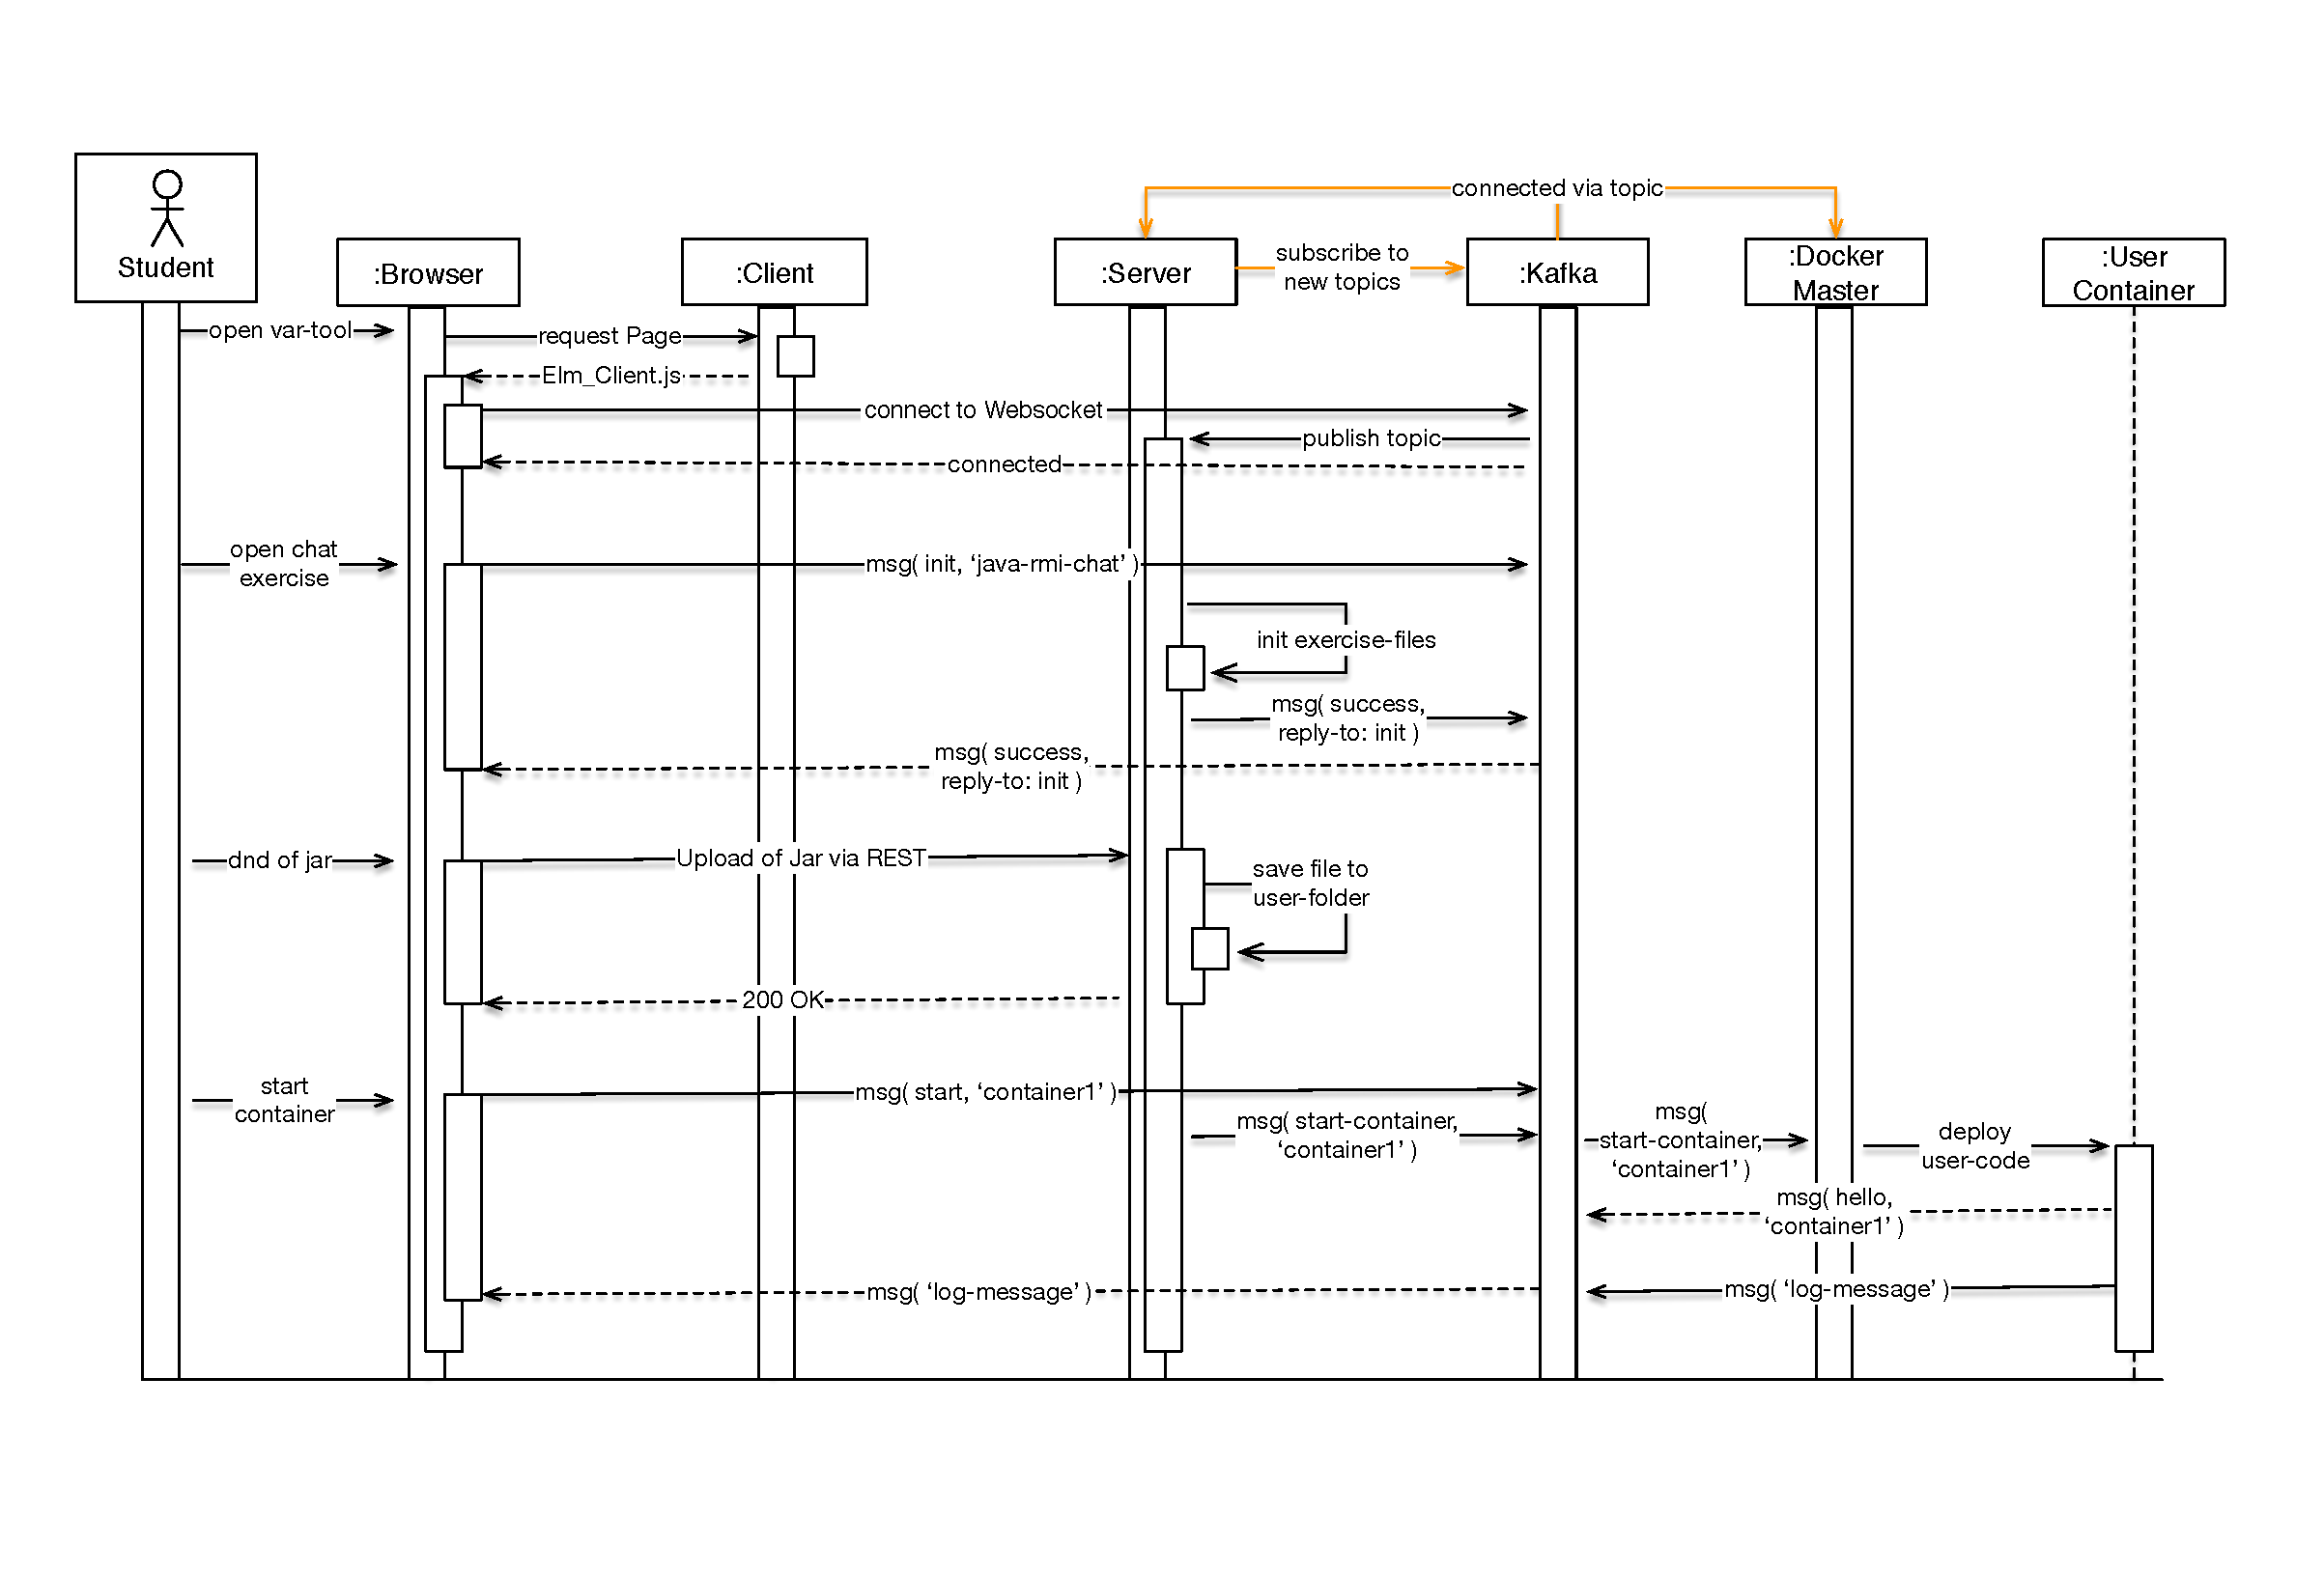
\includegraphics[scale=0.5]{sequence.pdf}
    \par
    \caption{Sequenzdiagramm}
    \label{fig:sequence}
  \end{figure}
\end{landscape}

\subsection{Netzwerkgrenzen}
  \begin{figure}[h]
    \centering
    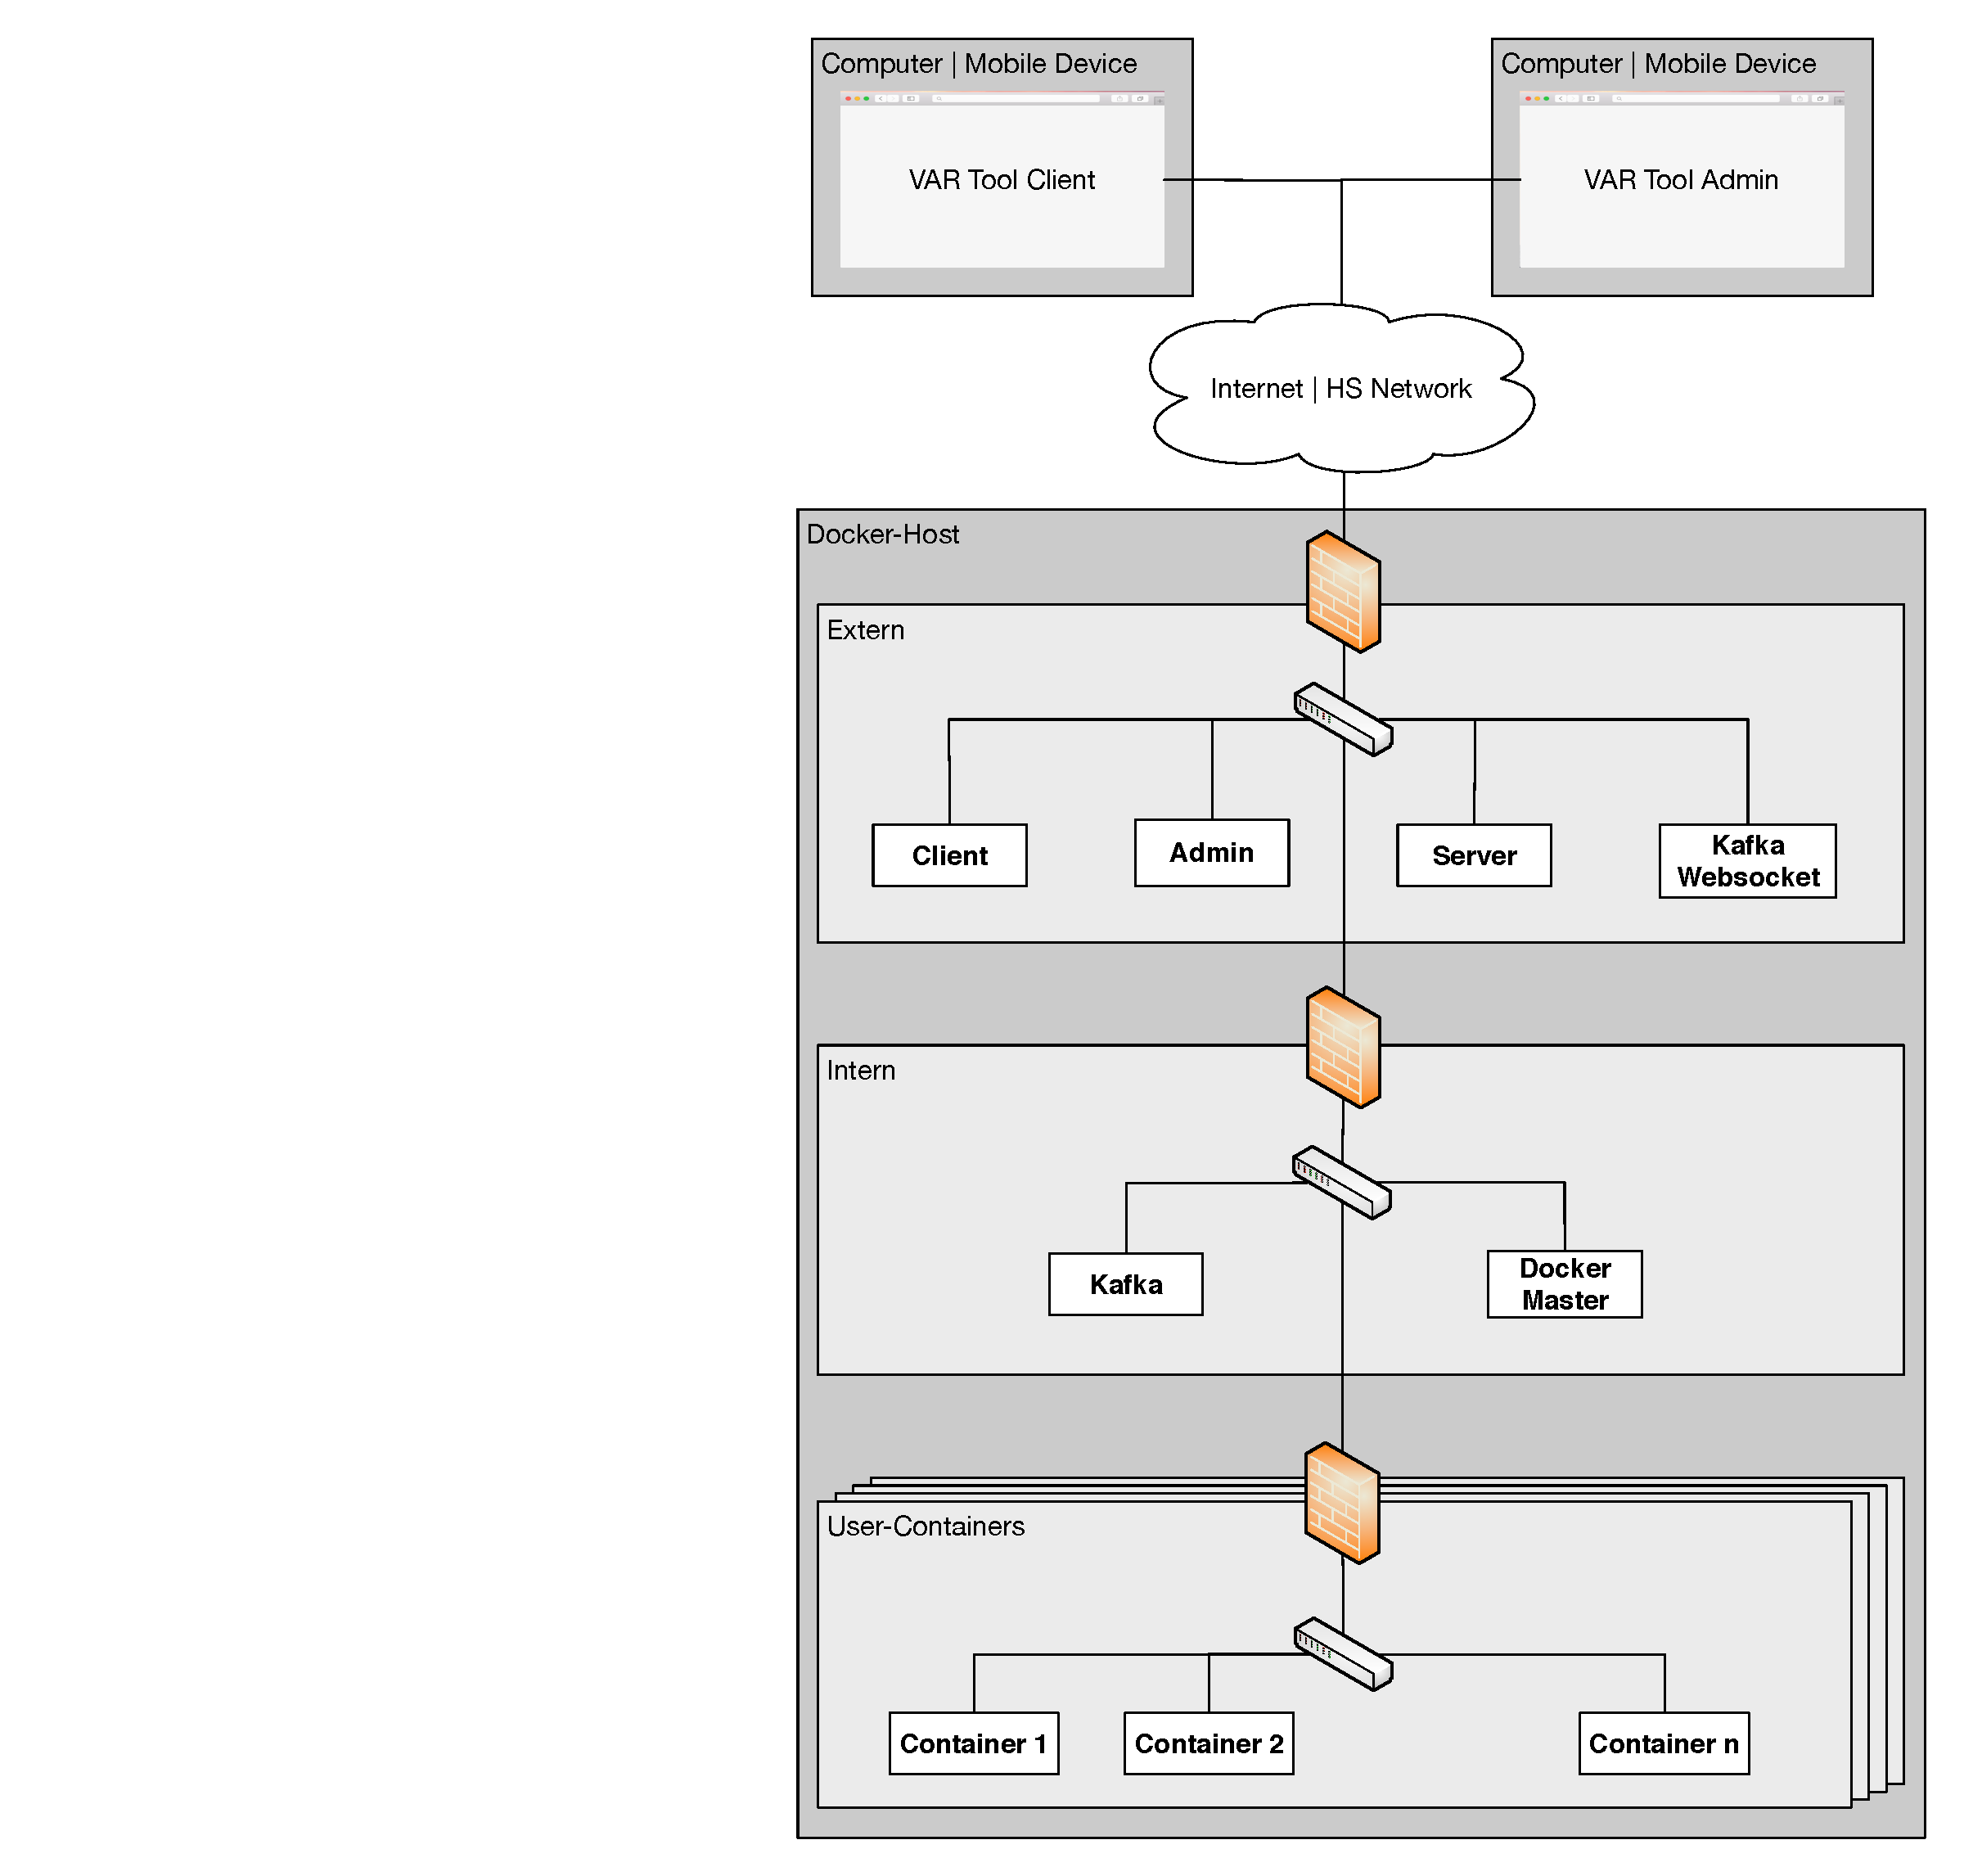
\includegraphics[scale=0.5]{network.pdf}
    \par
    \caption{Netzwerkdiagramm}
    \label{fig:network}
  \end{figure}

\subsection{Deployment}
\begin{landscape}
  \begin{figure}[h]
    \centering
    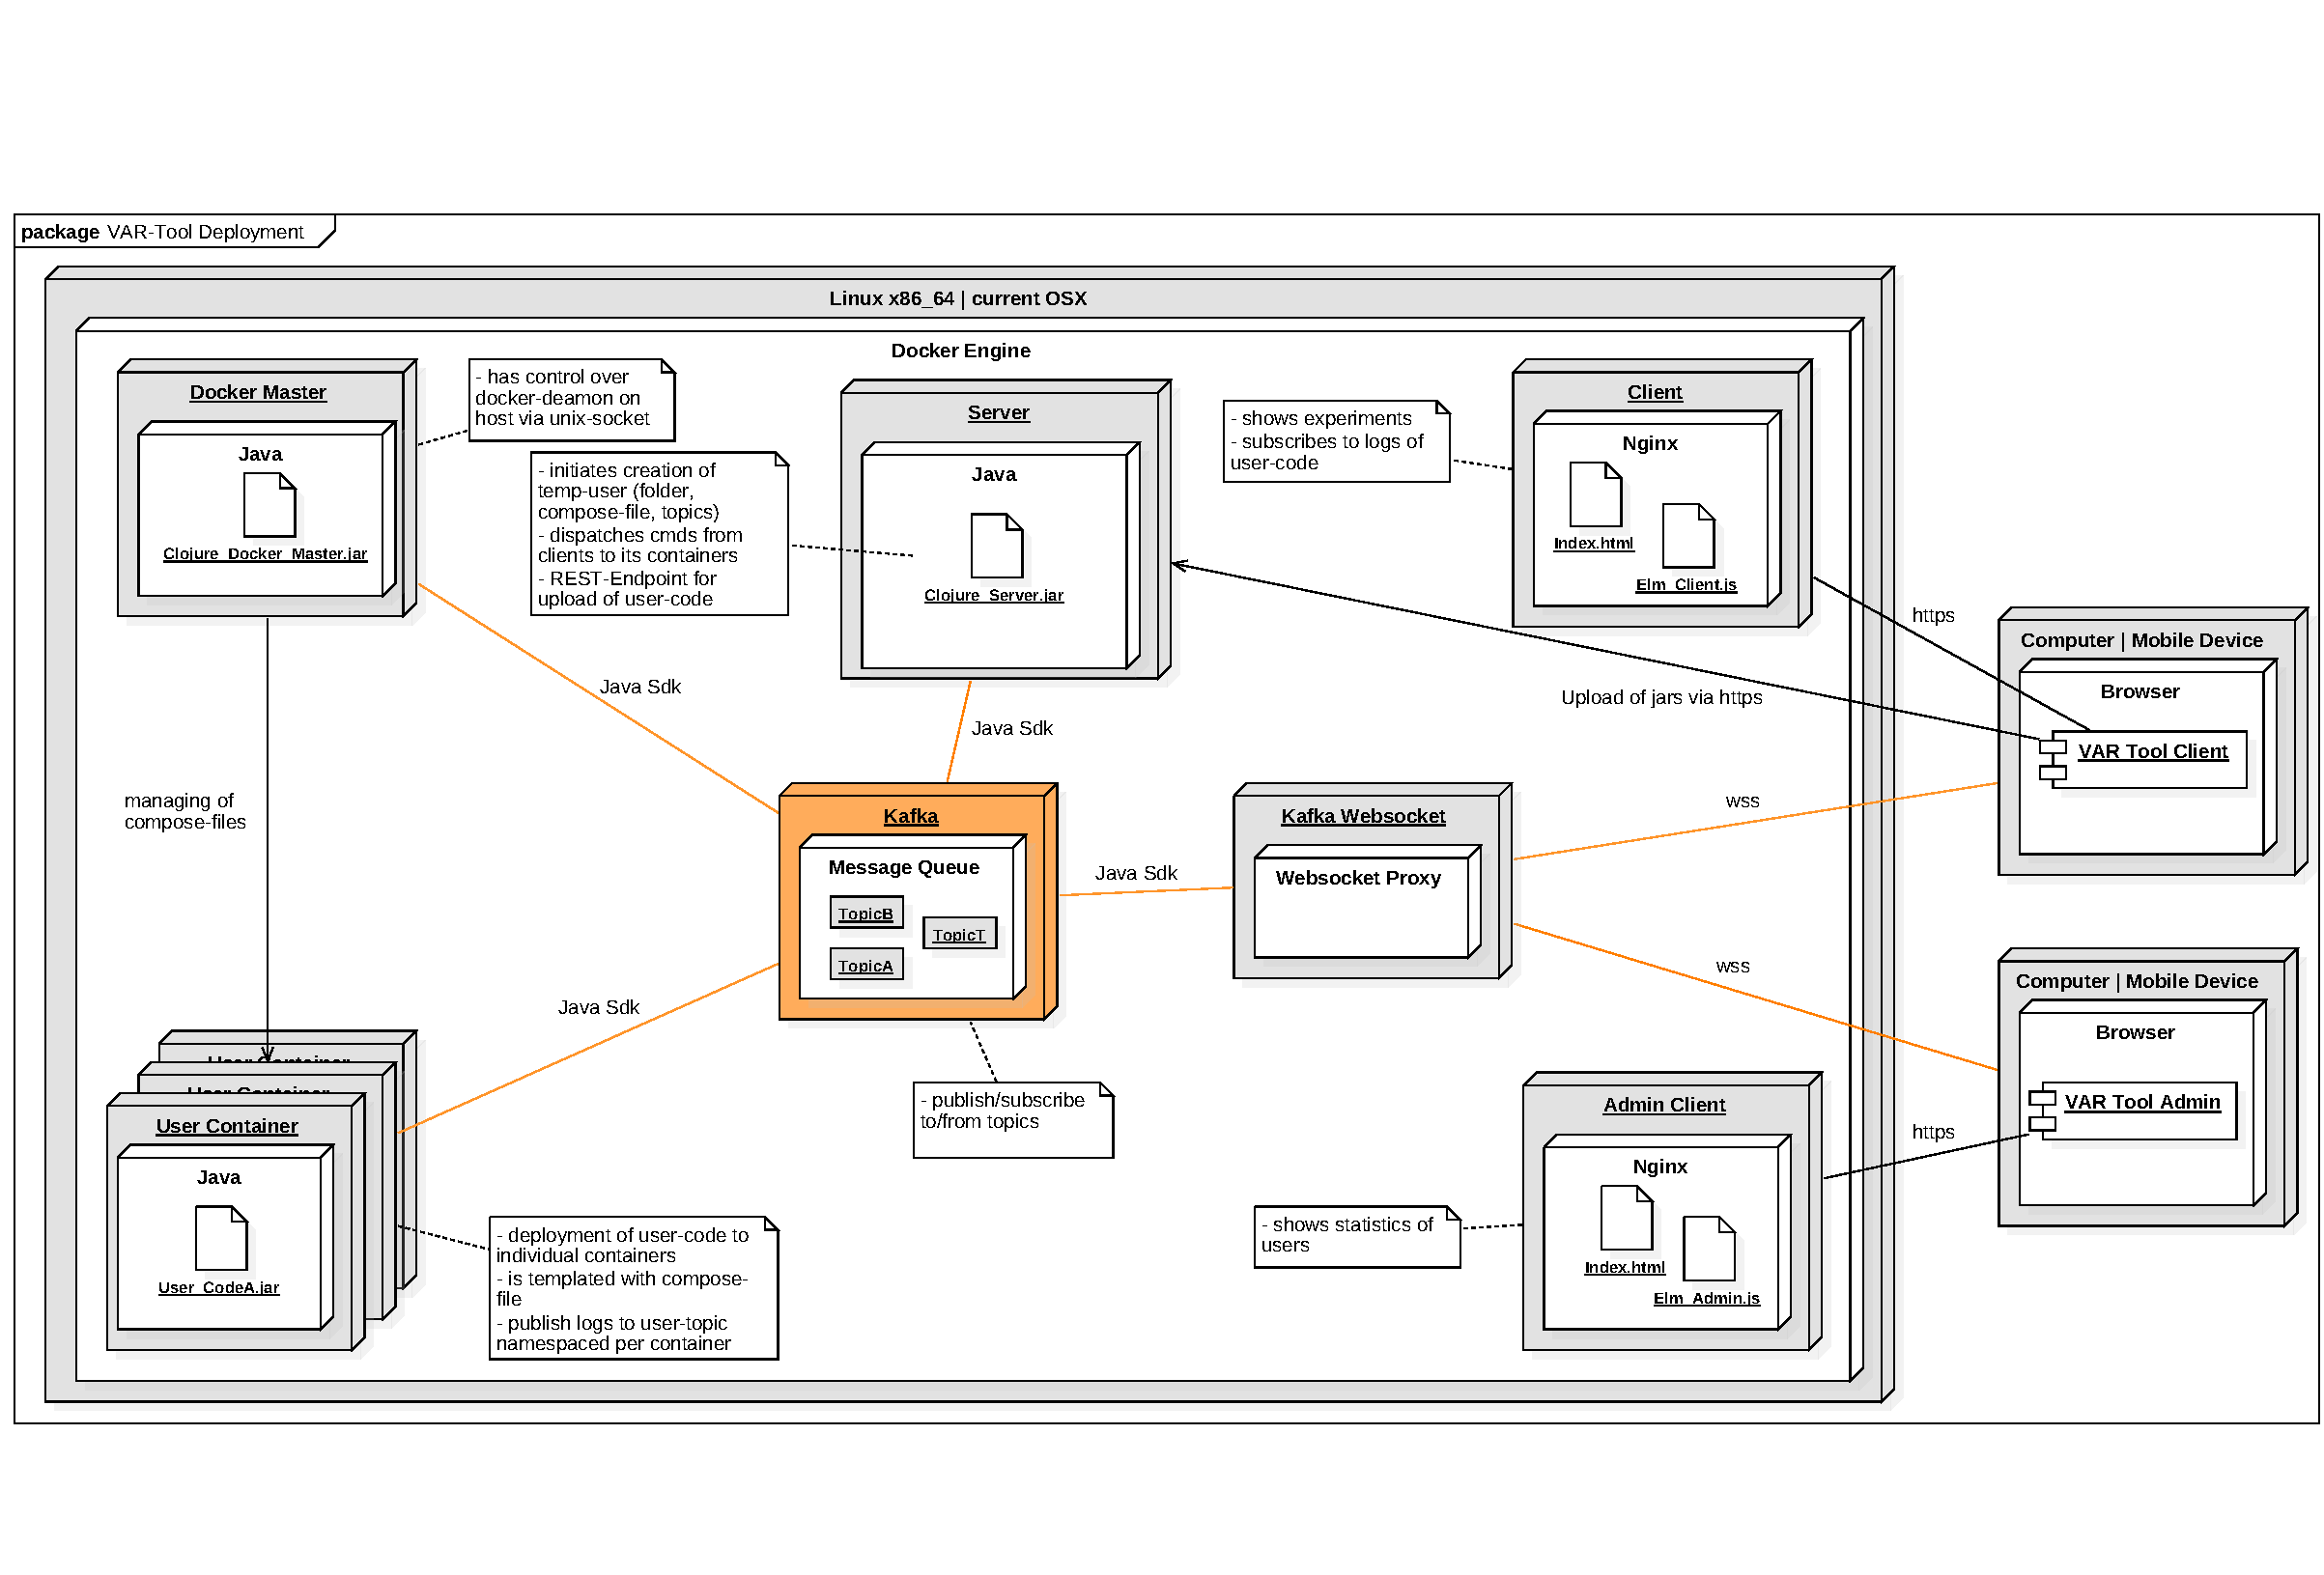
\includegraphics[scale=0.5]{deployment.pdf}
    \par
    \caption{Deploymentdiagramm}
    \label{fig:deployment}
  \end{figure}
\end{landscape}
\section{Umsetzung}
Im Folgenden werden Code-Beispiele gezeigt, welche in ihrem vollem Umfang im Repository des Projekts\footnote{\url{https://github.com/jwillem/var-tool}} zu finden sind.
\subsection{Kommunikation über Nachrichten}
Im Vorfeld wurde ein Nachrichten-Protokoll definiert, welches die Kommunikation zwischen Server und Client standardisiert.
Dabei heißen Client-Nachrichten \textit{Commands} und Server-Nachrichten \textit{Messages}.
So können beide Nachrichten-Typen durch ein triviales Merkmal unterschieden werden.
Jeweilig unterscheiden sich diese weiter in Kinder-Typen und deren \textit{Payloads}.
Dabei werden die Daten über eine Websocket-Verbindung in einem JSON-Envelope als String übertragen.
\\\\
\textbf{Commands:}
\begin{itemize}
  \item request-experiments:
    \\\texttt{\{ kind: command, \\subkind: request-experiments \}}
  \item add-input:
    \\\texttt{\{ kind: command, \\subkind: add-input,
    \\ payload: \{ experimentId: rmichat, \\\hspace*{1.8cm}instanceId: 1, \\\hspace*{1.8cm}input: Hello \}\}}
  \item start-instance:
    \\\texttt{\{ kind: command, \\ subkind: start-instance,
    \\ payload: \{ experimentId: rmichat, \\\hspace*{1.8cm}instanceId: 1, \\\hspace*{1.8cm}mainClass: var.rmi.chat.ChatClient, \\\hspace*{1.8cm}arguments: Anton \}\}}
  \item stop-instance:
    \\\texttt{\{ kind: command, \\ subkind: stop-instance,
    \\ payload: \{ experimentId: rmichat, instanceId: 1 \}\}}
\end{itemize}
\textbf{Messages:}
\begin{itemize}
  \item log:
    \\\texttt{\{ kind: message, \\subkind: log,
    \\ payload: \{ experimentId: rmichat, \\\hspace*{1.8cm}instanceId: 1, \\\hspace*{1.8cm}log: Hello\}\}}
  \item reply:
    \\\texttt{\{ kind: message, \\subkind: reply,
      \\ payload: \{ \\\hspace*{0.8cm}to: request-experiments, \\\hspace*{0.8cm}success: true, \\\hspace*{0.8cm}data: \{ \\\hspace*{1.6cm}rmichat: \{ \\\hspace*{2.4cm}id: rmichat, \\\hspace*{2.4cm}name: RMI Chat, \\\hspace*{2.4cm}lecturer: Sandro Leuchter, \\\hspace*{2.4cm}class: VAR, \\\hspace*{2.4cm}numberOfInstances: 4, \\\hspace*{2.4cm}instances: \{ \\\hspace*{3.2cm}1: \{ \\\hspace*{4cm}mainClass: var.rmi.chat.ChatClient, \\\hspace*{4cm}arguments: '' \\\hspace*{3.2cm}\}, .. \\\hspace*{2.4cm}\}\\\hspace*{1.6cm}\}, ..\\\hspace*{0.8cm}\}\\\}}
\end{itemize}
\clearpage

\subsection{Server}
Der Server besteht im Wesentlichen aus einem Webserver basierend auf \textit{http-kit} und \textit{ring} in der Programmiersprache Clojure.
Um die Entwicklung zu vereinfachen, wurde als erster Schritt ein Development-Container in Docker erstellt, welcher sich bei einer Änderung einer Quellendatei selbst aktualisiert, ohne die Java-VM neu zu starten. Es gibt dort drei Endpoints:
\begin{itemize}
  \item GET: \texttt{server:8080/hello}
    \\ Ankündigen des Clients am Server, Empfangen eines Responses mit \texttt{Set-Cockie}-Header
  \item \texttt{ws://server:8080/ws}
    \\ Anmeldung von Client an Websocket, Senden und Empfangen von Nachrichten
  \item POST: \texttt{server:8080/experiment/\{experimentId\}/instance/\{instanceId\}}
    \\ Hochladen der Programmpakete eines Studierenden
\end{itemize}
% \clearpage
Um auf eintreffende Nachrichten zu reagieren (\texttt{on-receive}), wurde eine \texttt{match}-Funktion innerhalb des Websocket-Handler genutzt (Listing 3.1).
Zunächst werden die Nachrichten von ihrer Json-Representation in ein für Clojure passendes Keyword decodiert.
Weiterhin wird auf eine passende verarbeitende Funktion verwiesen, oder einen Fehler mithilfe von \texttt{handle-\break command-error} an den Websocket-Channel zurückgegeben.
\par Bei einem Eintreffen eines \texttt{start-instance}-Commands wird ein Docker-Compose-Template eines Experiments mit den übergebenen Daten (Main-Class \& Argumentenliste) befüllt.
Dies geschieht mit dem Unix-Tool \texttt{envsubst} aus der \texttt{gettext}-Suite, welches Umgebungsvariablen in dem Docker-Compose-Template ersetzt.
Dabei wird die Datei als \texttt{docker-compose.yml} in dem Datenverzeichnis \texttt{data/submissions/\{session-token\}/} des Projekts gespeichert und ausgeführt (\texttt{docker-compose run user\_\{instanceId\}}).
Es wird zum Ausführen der jeweiligen Instanz das vorher hochgeladene Programmpaket in einem Unterordner mit dem Namen der Instanz-Id verwendet. 
\clearpage
\begin{verbatim}
(defn websocket-handler
  ""
  [request]
  (with-channel request channel
    (on-close
      channel
      (fn [status] (println "channel closed: " status)))
    (on-receive
      channel
      (fn [data]
        (let [session-token (get-in request [:cookies "ring-session" :value])
              ;; TODO error if session-token empty
              ;; TODO return error on java.lang.Exception: JSON error
              command-keyword (json/read-str data :key-fn keyword)
              _ (println "new command: " command-keyword)
              {:keys [kind subkind payload]} command-keyword]
          (match [kind subkind]
                 ["command" "request-experiments"]
                   (handle-request-experiments channel)
                 ["command" "add-input"]
                   (handle-add-input channel payload session-token)
                 ["command" "start-instance"]
                   (handle-start-instance channel payload session-token)
                 ["command" "stop-instance"]
                   (handle-stop-instance channel payload session-token)
                 :else (handle-command-error channel)))))))
\end{verbatim}
\begin{center}
  Listing 3.1: Websocket-Handler im Server (\texttt{handler.clj})
\end{center}
\clearpage

\subsection{Client}
Der Client wurde in der Programmiersprache Elm erstellt und nutzt \textit{elm-mdl} um die Darstellung aus Elementen im Stile des Material-Design Frameworks von Google aufzubauen.
Auch für den Client wurde zunächst ein Development-Container definiert, welcher automatisch neue Quelldateien kompiliert und den Browser dazu auffordert, sich zu aktualisieren.
\par
Die Entwicklung seiner Funktionen wurde stark durch das Typensystem und den Compiler von Elm geprägt, welche sich als sehr hilfreich herausgestellt haben.
Dazu wurden die Typen in einer Datei \texttt{Types.elm} definiert welche in anderen Elm-Modulen importiert wird.
Bei der Größe des Projekt ist es noch in Ordnung alle Typendefinitionen in einer Datei zu haben, jedoch sollte man diese in Zukunft bedachtsam in Unter-Module aufteilen.
\par
Weiterhin wurden die Json-Encoder definiert, welche ausgehende Nachrichten in eine Json-Representation bringt.
Ebenso war es wichtig eingehende Nachrichten mittels mehrerer Json-Decoder in Elm-Typen zu konvertieren.
Innerhalb dieser, konnte ebenso eine \texttt{match}-Funktion zum Einsatz gebracht werden (Listing 3.2).
Dabei können in einem \texttt{case}-Statement beliebige Elm-Typen auf einen Match überprüft werden.
Im Payload-Decoder wird ein Record vom Typ Message-Base mit dem \texttt{kind} von 'message' und den \texttt{subkind}s von 'log' oder 'reply' erwartet.
Im Code-Beispiel ist ebenso der Log-Payload-Decoder aufgeführt, welcher schließlich eine Log-Message zurückgibt.
\par Der vorbereitete Decoder kommt anschließend innerhalb der \texttt{update}-Funktion von \texttt{Update.elm} zum Einsatz (Listing 3.3).
Es wird zunächst überprüft, ob die Dekodierung erfolgreich war und anschließend den beiden Message-Typen zugeordnet, welche jeweilig anders mit den übergebenen Daten umgehen.
\par Die Umsetzung der Mockups aus Abbildung \ref{fig:ui-mockup-1} und \ref{fig:ui-mockup-2} sind in den Abbildungen \ref{fig:dev-view-1} und \ref{fig:dev-view-2} zu erkennen.
Dabei wurde versucht möglichst alle initialen Ideen zu erhalten und einige Verbesserungen integriert.
So war in den Mockups vorherig kein Eingabefeld vorhanden, um Eingaben an die laufenden Programme zu senden.
Weiterhin wurden die Zustände der Instanzansichten vereinfacht. Es sind nun folgende Zustände möglich:
\begin{itemize}
  \item Empty
    \\ Zeigt den File-Uploader
    (Abb. \ref{fig:dev-view-2} links oben)
  \item Uploading
    \\ Zeigt eine Warteinformation beim Hochladen der Programmpakete
    (Abb. \ref{fig:dev-view-2} rechts oben)
  \item Settings
    \\ Zeigt die Start-Parameter der Instanz
    (Abb. \ref{fig:dev-view-2} links unten)
  \item Running
    \\ Zeigt die Logs einer laufenden Instanz
    (Abb. \ref{fig:dev-view-2} rechts unten)
\end{itemize}
Die Darstellung der Instanzen aus Abbildung \ref{fig:dev-view-2} ist dynamisch, d.h. die Höhe der angezeigten Instanzen passt sich je nach Instanzanzahl eines Experiments an.
Somit wird die verfügbare Fläche des Browserfensters optimal genutzt.
\par Die angezeigten Experimente in Abbildung \ref{fig:dev-view-1} werden bei einem Neustart der Applikation über die bestehende Websocket-Verbindung abgefragt (request-experiments).
Die dabei erhaltenen Daten werden im Browser-Cache gespeichert und können nach einem Auswählen eines Experiments wiederverwendet werden.
\clearpage
\begin{verbatim}
messageDecoder : Decoder Message
messageDecoder =
    map2 MessageBase
        (field "kind" string)
        (field "subkind" string)
        |> andThen payloadDecoder

payloadDecoder : MessageBase -> Decoder Message
payloadDecoder { kind, subkind } =
    case kind of
        "message" ->
            case subkind of
                "log" ->
                    field "payload" logPayloadDecoder

                "reply" ->
                    field "payload" replyPayloadDecoder

                _ ->
                    fail "Subkind is unknown!"

        _ ->
            fail "Kind is unknown!"


logPayloadDecoder : Decoder Message
logPayloadDecoder =
    map3 LogPayload
        (field "experimentId" string)
        (field "instanceId" string)
        (field "log" string)
        |> andThen logMessageDecoder


logMessageDecoder : LogPayload -> Decoder Message
logMessageDecoder payload =
    succeed (LogMessage payload)
\end{verbatim}
\begin{center}
  Listing 3.2: Json-Decoder der Log-Messages im Client (\texttt{Decoders.elm})
\end{center}
\clearpage
\begin{verbatim}
handleNewMessage : Model -> String -> ( Model, Cmd Msg )
handleNewMessage model message =
    let
        decodedMessage =
            Decoders.decodeMessage message
    in
        case decodedMessage of
            Ok message ->
                case message of
                    LogMessage payload ->
                        handleLogMessage model payload

                    DataMessage payload ->
                        handleDataMessage model payload

            Err error ->
                let
                    _ =
                        Debug.log "Decoder" error
                in
                    ( model, Cmd.none )
\end{verbatim}
\begin{center}
  Listing 3.3: Verarbeiten von neuen Nachrichten im Client (\texttt{Update.elm})
\end{center}

\begin{landscape}
  \begin{figure}[h]
    \centering
    \fbox{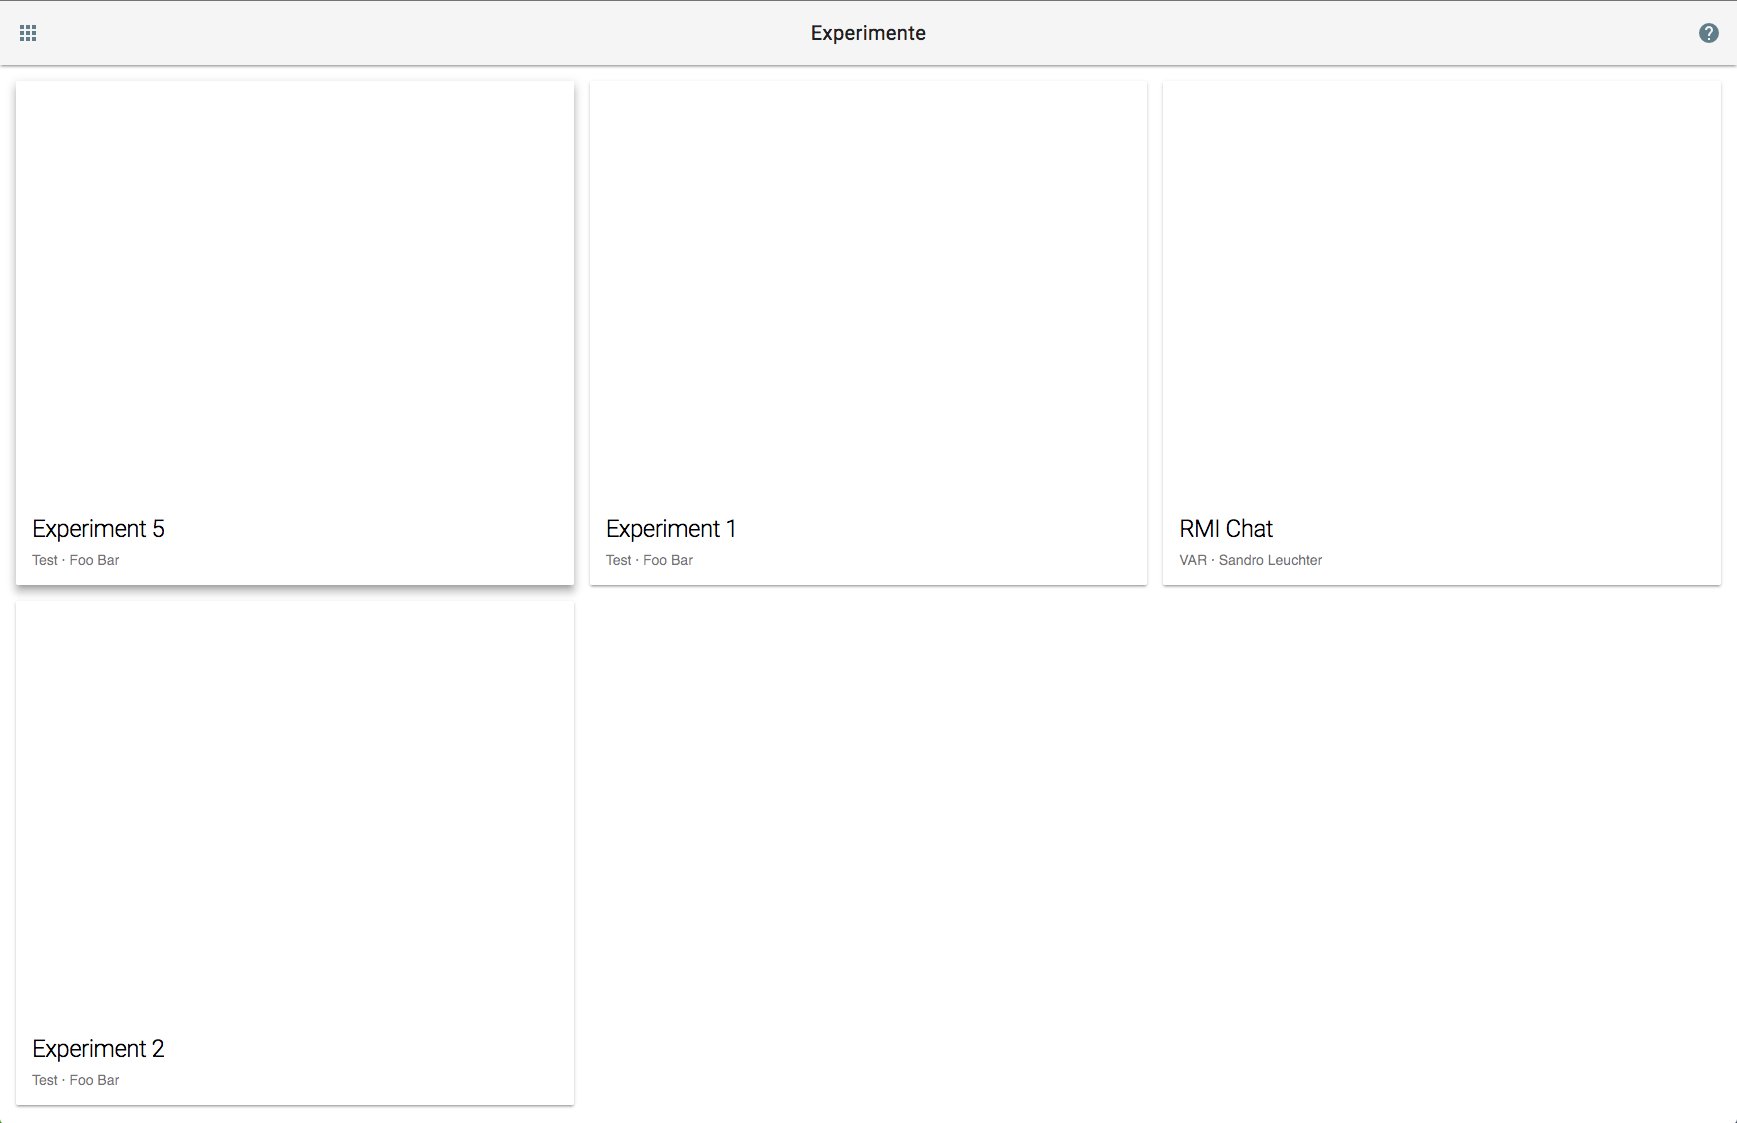
\includegraphics[scale=0.35]{current_dev_view_overview.png}}
    \par
    \caption{Umsetzung des Clients: Übersichtsseite}
    \label{fig:dev-view-1}
  \end{figure}
  \begin{figure}[h]
    \centering
    \fbox{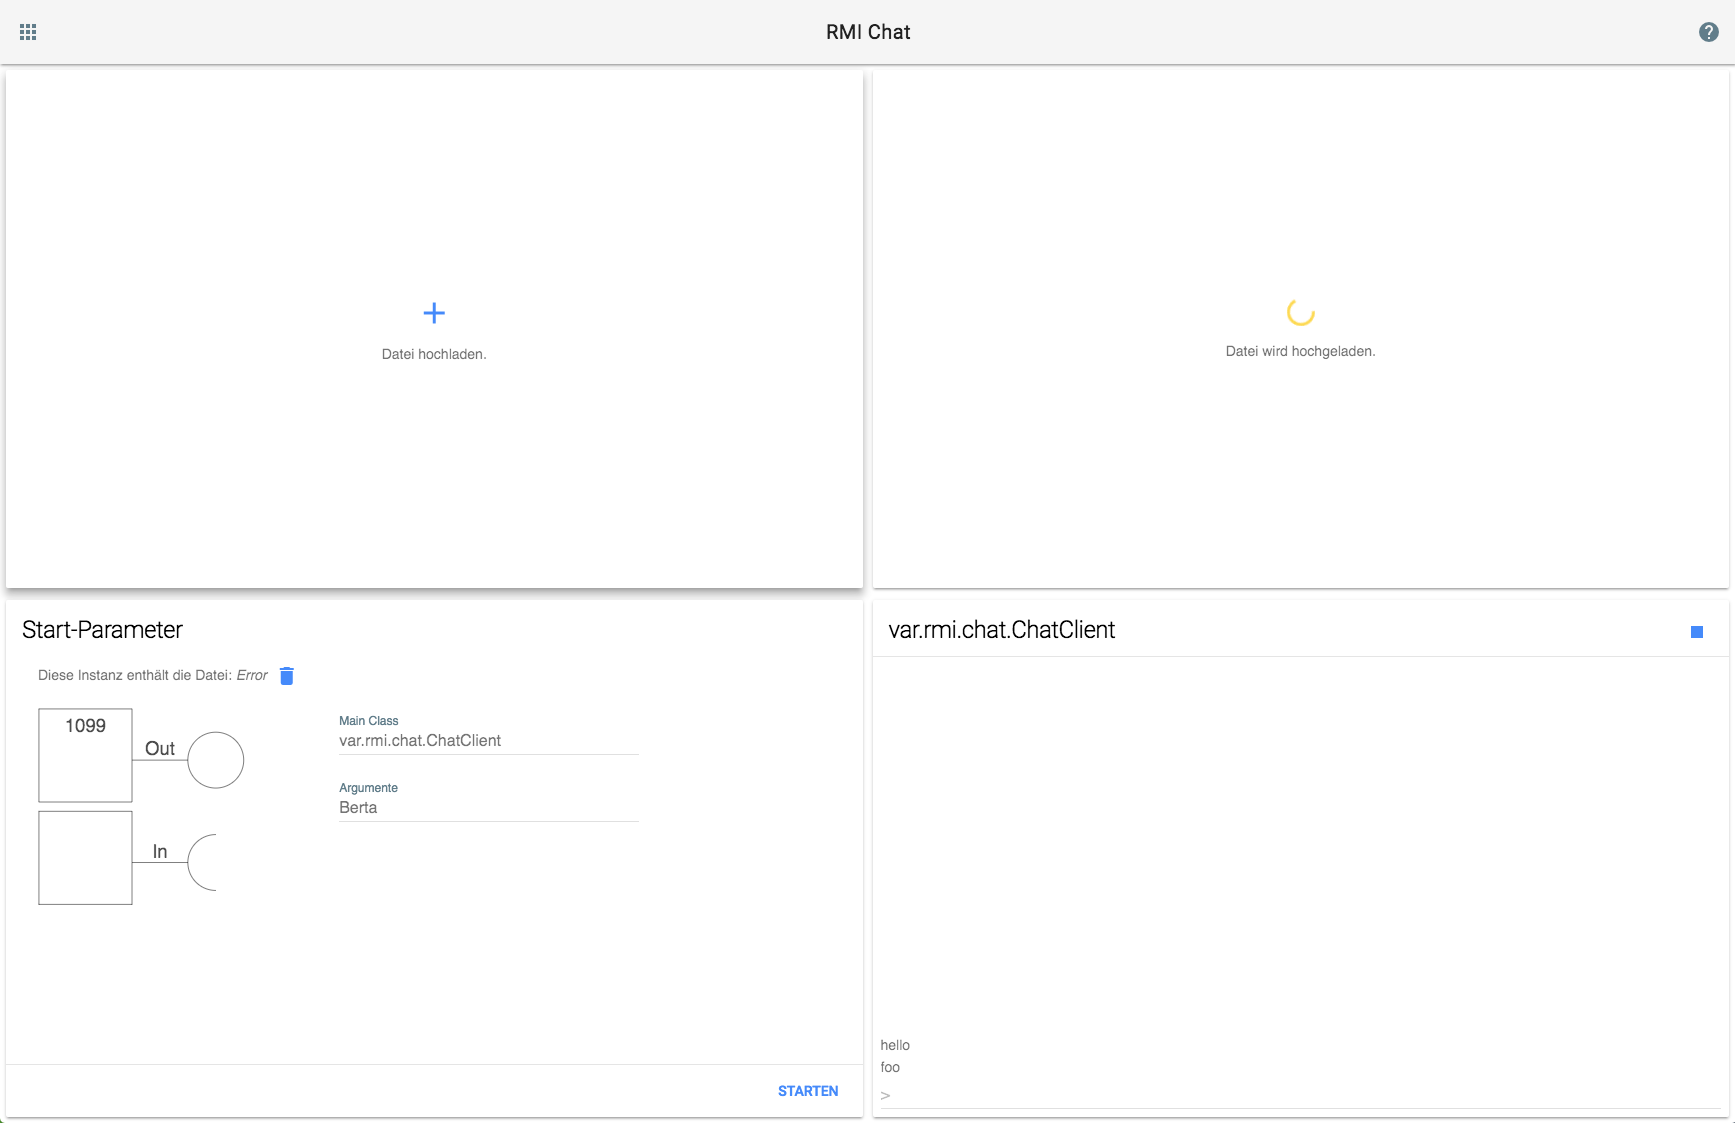
\includegraphics[scale=0.35]{current_dev_view_experiment.png}}
    \par
    \caption{Umsetzung des Clients: Experimentenansicht}
    \label{fig:dev-view-2}
  \end{figure}
\end{landscape}
\section{Erwartungen an die Performance}
\section{Installation}
Als erstes wird das Projekt mithilfe von \texttt{git clone \url{https://github.com/jwillem/var-tool.git}} heruntergeladen.
Um die Applikation zu starten, werden zunächst die Installationen von Docker\footnote{\url{https://www.docker.com/community-edition}} und Docker-Compose\footnote{\url{https://docs.docker.com/compose/install/}} benötigt.
Nach einem Ausführen von \texttt{docker-compose build} im Projektverzeichnis kann die App mit \texttt{docker-compose up} gestartet werden.
